% !TEX root = Séquence 2 - Activités - Vecteurs.tex
% Transcription de l'activité 3 (Enchaîner deux translations) du manuel,
% en autonome (même montage que "Séquence 2 - Cours - Vecteurs.tex" : on
% recharge CLT2627.sty par \input direct à cause de l'espace dans le nom
% du dossier).
\documentclass[a4paper,11pt,french]{report}
\input{../TeX - Polycopié et Exercices/CLT2627.sty}
\graphicspath{{../TeX - Polycopié et Exercices/}}

\usetikzlibrary{shapes.misc, arrows.meta}
\tikzset{cross/.style={cross out, draw=black, minimum size=#1, inner sep=0pt}}

\begin{document}
\pagestyle{empty}

\newtcolorbox{JauneBox}{enhanced,colback=yellow!12,colframe=yellow!55!black,
  boxrule=0.6pt,arc=2pt,left=6pt,right=6pt,top=4pt,bottom=4pt}

% Point représentant le palet : petit cercle avec une croix à l'intérieur.
\newcommand{\Palet}[1]{\node[draw,circle,inner sep=1.3pt] at #1 {\tiny$+$};}


\begin{center}
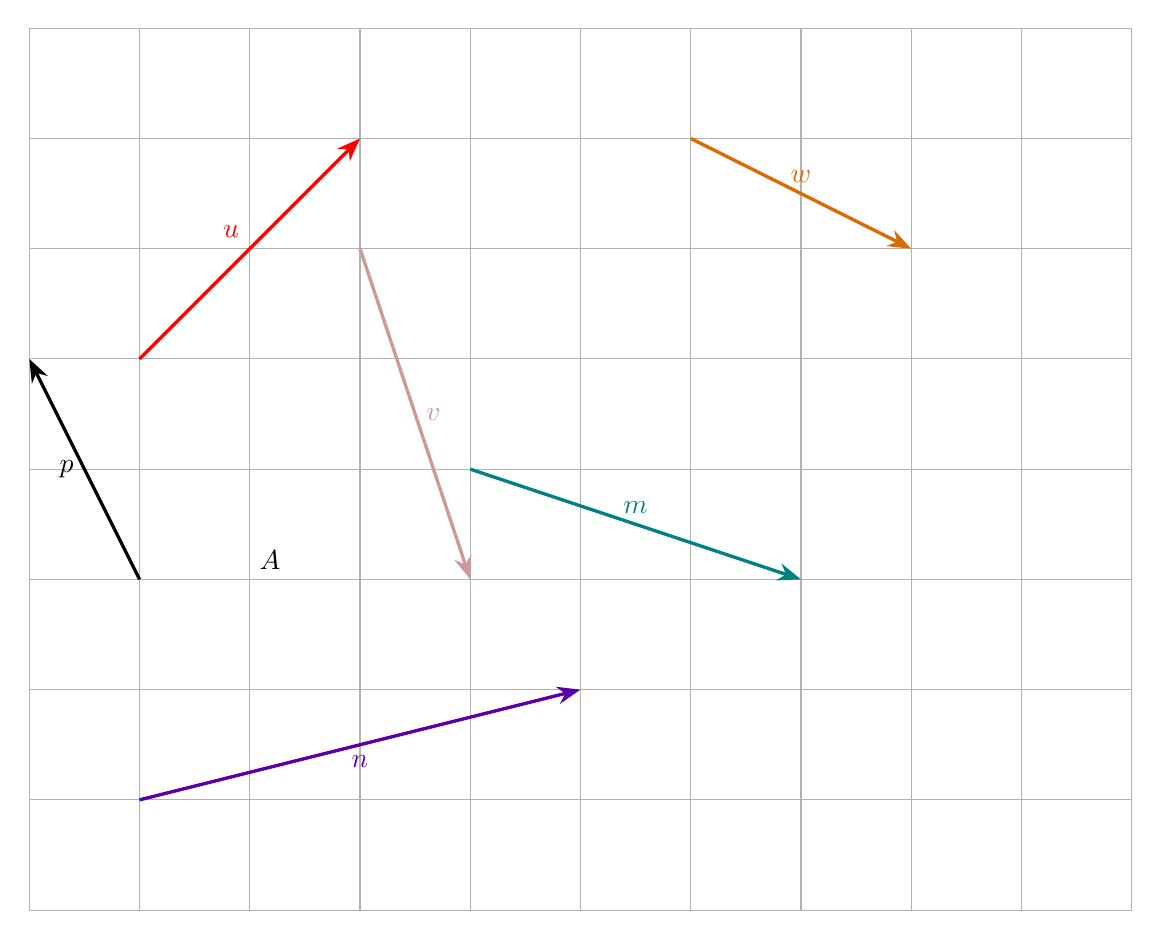
\begin{tikzpicture}[scale=1.4, >=Stealth]
\draw[thin,gray!60] (0,0) grid (10,8);
\Palet{(2,3)} \node[above right] at (2,3) {$A$};

\draw[->,very thick,red] (1,5) -- (3,7) node[midway,above left]{$\Vj u$};
\draw[->,very thick,orange!85!black] (6,7) -- (8,6) node[midway,above]{$\Vj w$};
\draw[->,very thick,violet!70!blue] (1,1) -- (5,2) node[midway,below]{$\Vj n$};
\draw[->,very thick,teal] (4,4) -- (7,3) node[midway,above]{$\Vj m$};
\draw[->,very thick,pink!80!black] (3,6) -- (4,3) node[midway,right]{$\Vj v$};
\draw[->,very thick,black] (1,3) -- (0,5) node[midway,left]{$\Vj p$};
\end{tikzpicture}
\end{center}

\bigskip

\bigskip

\begin{center}
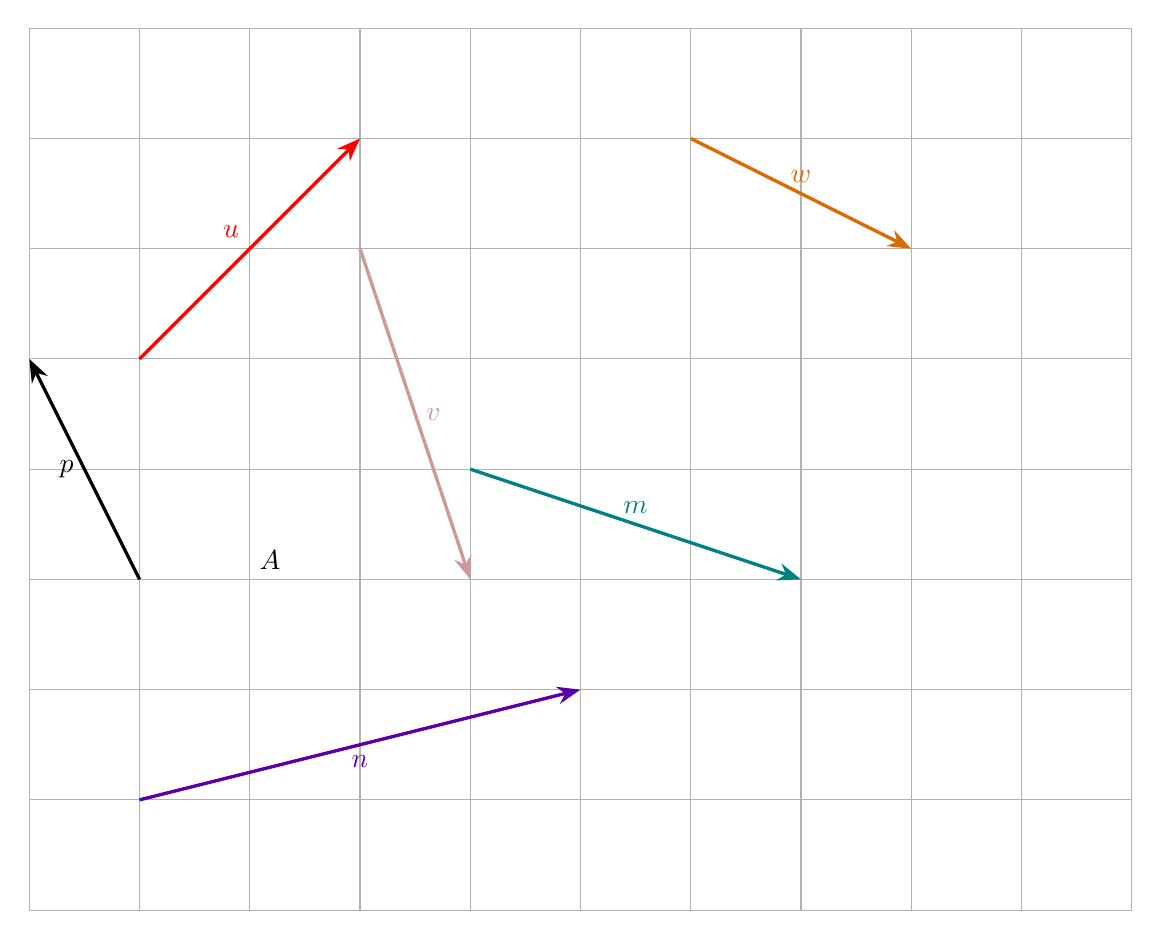
\begin{tikzpicture}[scale=1.4, >=Stealth]
\draw[thin,gray!60] (0,0) grid (10,8);
\Palet{(2,3)} \node[above right] at (2,3) {$A$};

\draw[->,very thick,red] (1,5) -- (3,7) node[midway,above left]{$\Vj u$};
\draw[->,very thick,orange!85!black] (6,7) -- (8,6) node[midway,above]{$\Vj w$};
\draw[->,very thick,violet!70!blue] (1,1) -- (5,2) node[midway,below]{$\Vj n$};
\draw[->,very thick,teal] (4,4) -- (7,3) node[midway,above]{$\Vj m$};
\draw[->,very thick,pink!80!black] (3,6) -- (4,3) node[midway,right]{$\Vj v$};
\draw[->,very thick,black] (1,3) -- (0,5) node[midway,left]{$\Vj p$};
\end{tikzpicture}
\end{center}


\newpage 

\begin{landscape}

\begin{center}
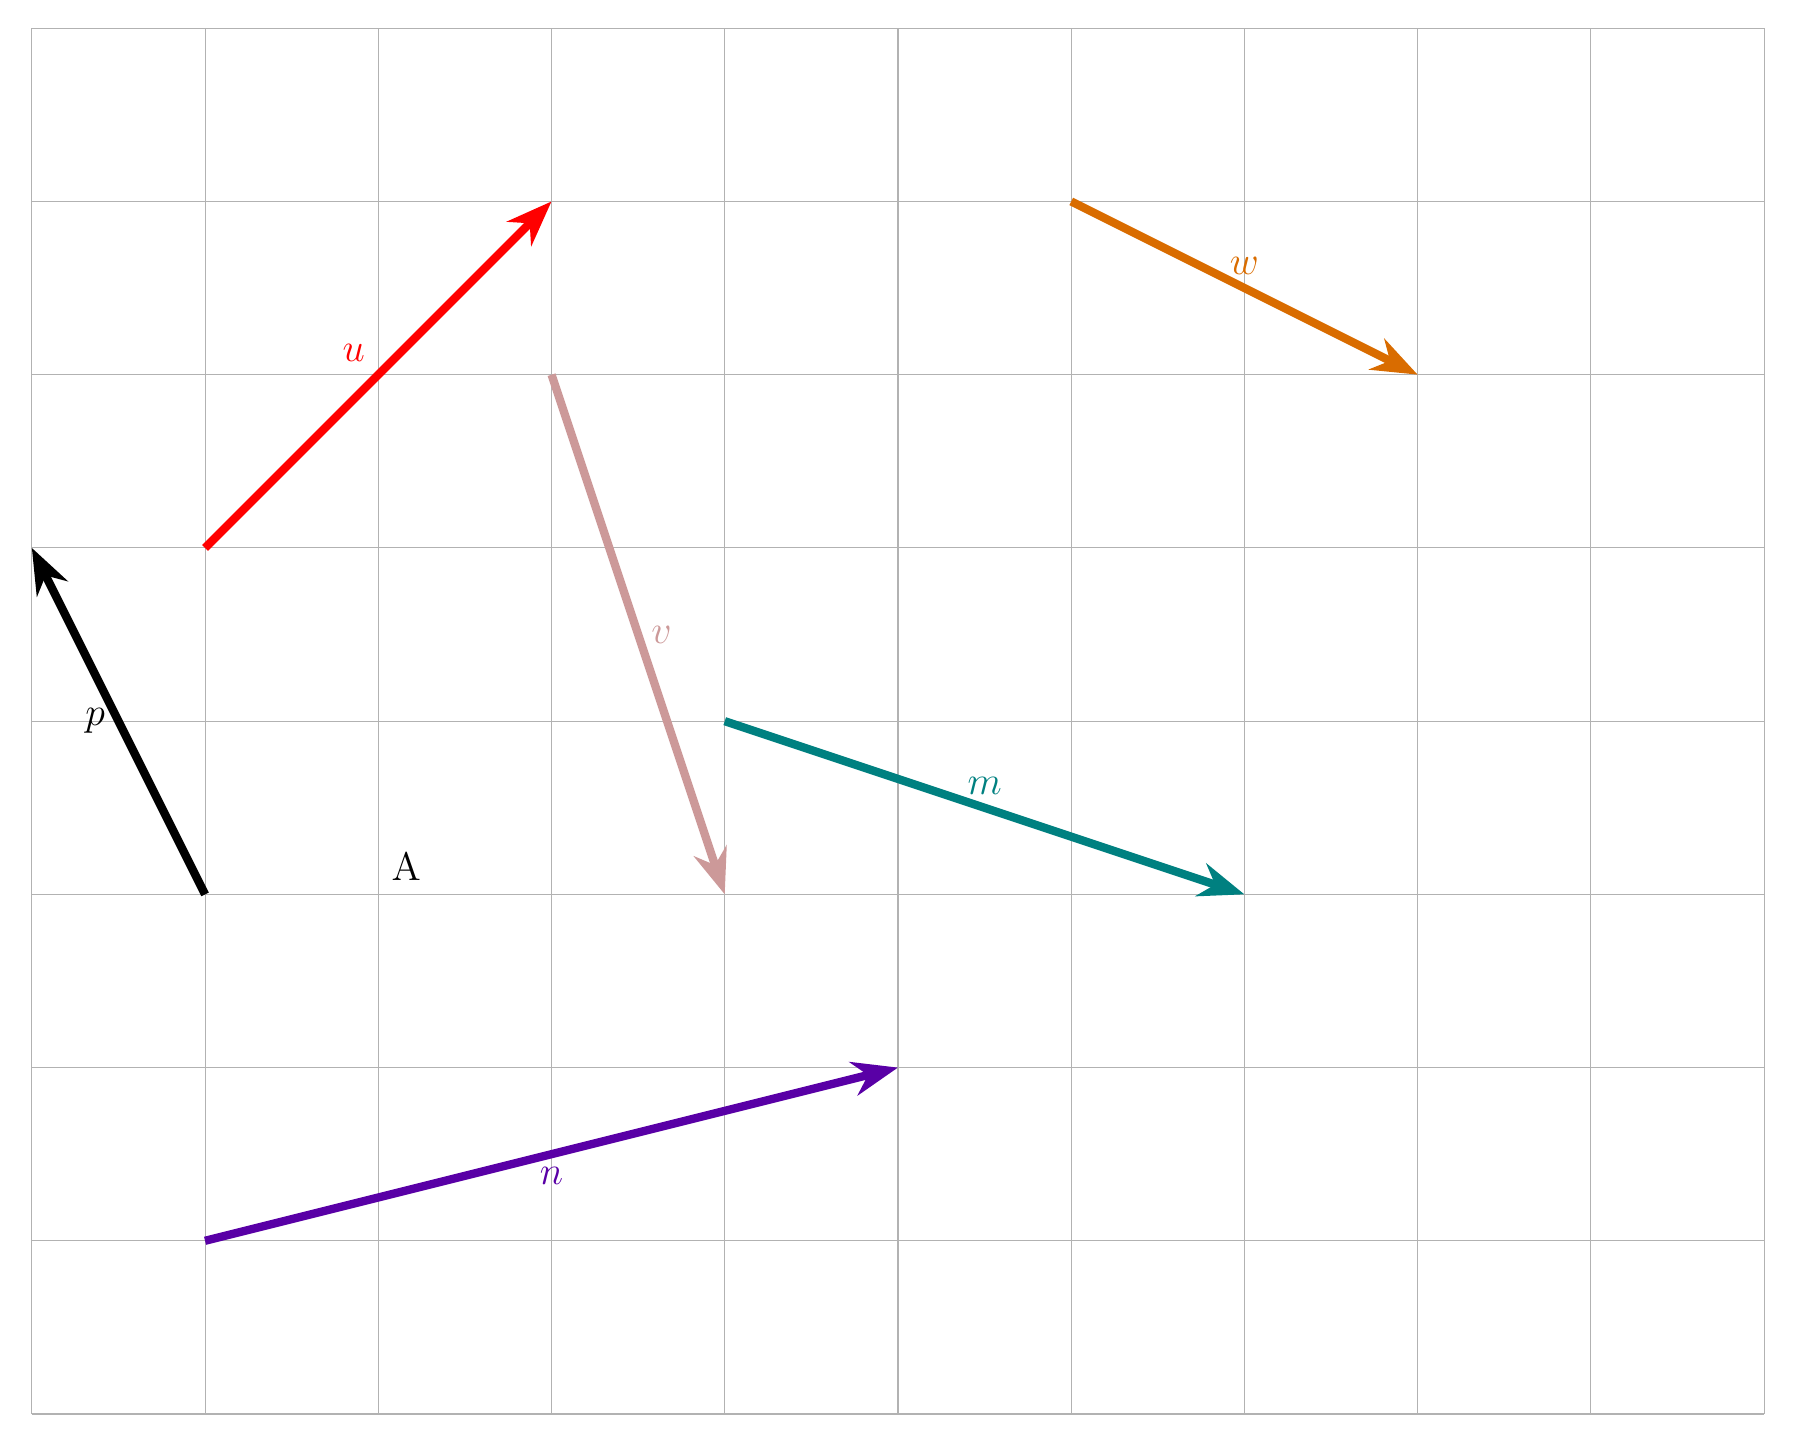
\begin{tikzpicture}[
  scale=2.2, 
  >=Stealth, 
  line width=3pt, % Définit une épaisseur personnalisée pour tous les traits
  nodes={font=\Large} % Applique \large à tous les nœuds de la figure
]
\draw[thin,gray!60] (0,0) grid (10,8);
\Palet{(2,3)} \node[above right] at (2,3) {A};

\draw[->,red] (1,5) -- (3,7) node[midway,above left]{$\Vj u$};
\draw[->,orange!85!black] (6,7) -- (8,6) node[midway,above]{$\Vj w$};
\draw[->,violet!70!blue] (1,1) -- (5,2) node[midway,below]{$\Vj n$};
\draw[->,teal] (4,4) -- (7,3) node[midway,above]{$\Vj m$};
\draw[->,pink!80!black] (3,6) -- (4,3) node[midway,right]{$\Vj v$};
\draw[->,black] (1,3) -- (0,5) node[midway,left]{$\Vj p$};
\end{tikzpicture}
\end{center}

\end{landscape}



\end{document}
